\documentclass[10pt,a4paper]{article}
\usepackage[utf8]{inputenc}
\usepackage[portuguese]{babel}
\usepackage{titlesec}
\usepackage{graphicx}
\usepackage{indentfirst}
\usepackage{enumerate}
\usepackage{float}
\usepackage{array}
\usepackage{tikz}
\usepackage{multirow}
\usepackage{multicol}
\usepackage{geometry}
\usepackage[cache=false]{minted}
\usepackage{pdflscape}
\usepackage[titletoc]{appendix}
\usepackage{hyperref}
\geometry{
 a4paper,
 top=2cm,
 bottom=2cm,
 left=3cm,
 right=3cm
}
\addto\captionsportuguese{
      \renewcommand{\contentsname}
          {Índice}
}

\begin{document}
\begin{titlepage}
    \center
    {\huge {\bf Universidade do Minho}}\\[0.4cm]
    \vspace{3.0cm}
    \textsc{\huge{Java Factura}}\\[0.5cm]
    \vspace{3.0cm}
    \textsc{\huge{Mestrado Integrado em Engenharia Informática}}\\[0.5cm]
    \vspace{2.0cm}
    \textsc{Programação Orientada a Objectos}\\[0.5cm]
    \textsc{(2º Ano, 2º Semestre, 2017/2018)}\\[0.5cm]
    \vspace{1.5cm}
    \begin{flushleft}
        Grupo 11
        \vspace{1cm}

        A79003 \,\,\,Pedro Mendes Félix da Costa
    \end{flushleft}
        \vspace{1cm}
    \begin{flushright}
        Braga

        Maio 2018
    \end{flushright}

\end{titlepage}

\tableofcontents
\clearpage

\section{Introdução}
    Este trabalho foi realizado no âmbito da unidade curricular programação
    orientada a objectos e teve como objetivo a implementação de um sistema
    similar ao \href{www.efactura.pt}{EFatura} aplicando os conceitos
    lecionados nas aulas.

\section{Principais entidades do Sistema}
    \subsection{User}
    A interface \textbf{User} é implementada por duas classes, \textbf{Admin} e
    \textbf{Contribuinte}. Esta ultima, sendo um classe abstrata é ainda
    estendida por \textbf{ContribuinteEmpresarial} e
    \textbf{ContribuinteIndividual}.

    \begin{figure}[h]
        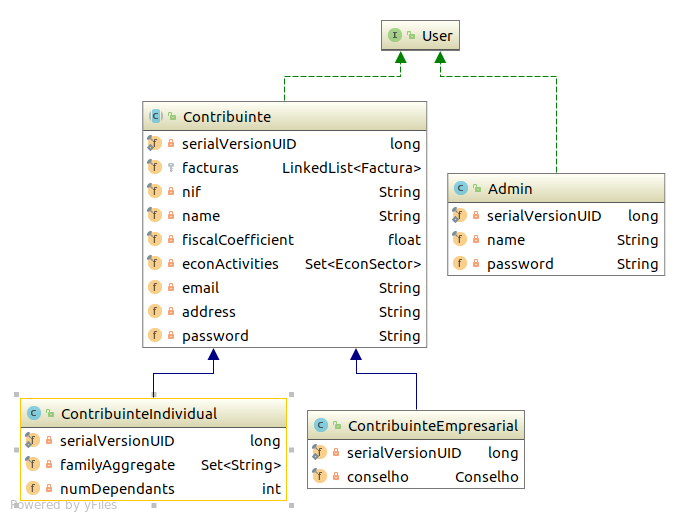
\includegraphics[width=\textwidth]{./images/UserHierarquy.png}
    \end{figure}

    Um \textbf{User} tem obrigatoriamente de implementar
    \begin{multicols}{3}
    \begin{itemize}
        \item \mintinline{java}{getNif()}
        \item \mintinline{java}{getName()}
        \item \mintinline{java}{getPassword()}
        \item \mintinline{java}{setPassword()}
        \item \mintinline{java}{clone()}.
    \end{itemize}
    \end{multicols}
    Um \textbf{Admin} implementa apenas a interface, não adicionando mais
    nenhuma funcionalidade, note-se, no entanto, que o nif e nome do admin são
    sempre iguais a "\mintinline{java}{admin}".

    A classe \textbf{Contribuinte} para além de implementar a interface
    guarda também como variaveis o email, morada, coeficiente fiscal, sectores
    de actividade economica, as facturas. Estes ultimos dois atributos são
    vistos de forma diferente dependendo da subclasse que a extende.

    O \textbf{ContribuinteEmpresarial} acrescenta ao \textbf{Contribuinte}
    o \textbf{Conselho} onde reside, este podendo ser do interior ou não. Para
    além disto vê as suas facturas como as vendas que realizou os sectores de
    actividade economica como os possiveis sectores que as facturas que emite
    podem tomar.

    O \textbf{ContribuinteIndividual} acrescenta ao \textbf{Contribuinte}
    o agregado familiar e número destes que são dependentes. Este vê as suas
    facturas como as suas despesas e os sectores economicos como os sectores
    de onde pode deduzir das facturas.

    \subsection{Factura}

    Fazendo uma análise às queries, decidimos que seria necessário representar
    as seguintes entidades:

    \subsection{Posts}
    Para representar os \textbf{posts} dividimos os atributos por duas
     sub estruturas, cujos atributos de cada uma das sub estruturas são:
        \subsubsection{Questões}
        \begin{multicols}{2}
        \begin{itemize}
            \item Id
            \item Score
            \item Data
            \item Título da questão
            \item Id do autor da questão
            \item Nome do autor da questão
            \item Número de respostas
            \item Lista das respostas
            \item Tags
        \end{itemize}
        \end{multicols}

        \subsubsection{Respostas}
        \begin{multicols}{2}
        \begin{itemize}
            \item Id
            \item Score
            \item Data
            \item Número de comentários
            \item Id do autor da resposta
            \item Id da questão a que responde
            \item Nome do autor da resposta
            \item Referência da questão a que responde
        \end{itemize}
        \end{multicols}
    Além dos dados fornecidos diretamente pelos ficheiros xml, decidimos também
    guardar na \textbf{questão} a lista das \textbf{respostas} de cada questão,
    bem como uma contagem destas. Na \textbf{resposta}, inversamente, guardamos
    uma referência para a pergunta a que esta responde. Com estas informações
    extra as pesquisas que envolvem relacionar estas duas entidades tornam-se
    mais eficientes.

        \subsubsection{Post}
        Ambas estas estruturas, questões e respostas, podem ser representadas de
        forma abstrata por um \textbf{Post}.

        Esta estrutura é necessária, pois o utilizador precisa de guardar
        todas as questões e respostas, sem ser necessário uma distinção entre
        os dois tipos.

    \subsection{Utilizadores}
    Para representar os \textbf{utilizadores} guardamos os seguintes atributos:
    \begin{multicols}{3}
    \begin{itemize}
            \item Id
            \item Biografia
            \item Nome
            \item Reputação
            \item Número de posts
            \item Lista dos posts
    \end{itemize}
    \end{multicols}
    Mais uma vez foram guardadas mais informações para além das disponibilizadas
    diretamente pelo xml. Foi guardado o número de \textbf{posts} do utilizador
    (para determinar os utilizadores mais ativos de forma mais rápida) e a lista
    destes para permitir pesquisas mais rápidas.

\section{Estruturas de Dados}
    \subsection{Tipo concreto de dados}
    Para armazenar as entidades descritas acima foi implementado um TCD que
    as armazena de diferentes formas.
    \begin{minted}{C}
struct TCD_community{
    QUESTIONS_HTABLE questions;
    ANSWERS_HTABLE answers;
    SO_USERS_HTABLE users;
    TAGS_HTABLE tags;
    CALENDARIO calendarioQuestions;
    CALENDARIO calendarioAnswers;
};
    \end{minted}
    \subsection{Hashtables}
        Todas as entidades são armazenadas numa tabela de hash pois para todas
        são necessárias pesquisas por id (ou nome no caso das tags).

        \subsubsection{Tags}
        A tabela de hash das \textit{tags} serve para criar uma associação
        $Nome \to Id$ visto que as questões guardam uma lista com os nomes das
        tags e para responder à query 11 é necessário obter os ids das mesmas.

    \subsection{Calendário}
        Para ser possivel manter as questões e respostas ordenadas por data
        foi pensada a utilização de árvores binárias ordenadas por data,
        mas isto foi considerado ineficiente quando comparada à solução
        escolhida. Foi então concebida uma estrutura à qual demos o nome
        de \textbf{Calendário} que permite acessos em tempo constante $O(1)$
        a todos os elementos associados a uma determinada data. Guardamos assim
        duas instâncias desta na TCD, uma para perguntas e outra para respostas.

        Esta estrutura permite:
        \begin{itemize}
                \item Guardar qualquer objeto desde que seja
                      passada uma data associada ao mesmo.
                \item Iterar sobre os objetos, dado um intervalo de tempo,
                      por ordem cronológica normal ou inversa, conforme a
                      ordem dos argumentos.
        \end{itemize}

        A estrutura em si consiste numa matriz de quatro dimensões com um lista
        ligada em cada célula desta.

        No primeiro nível temos uma lista de \textbf{anos}. Cada um destes,
        é constituído por uma lista de \textbf{meses} que são constituídos por
        uma lista de \textbf{dias}, cujo tamanho varia entre 29 e 31. Cada
        \textbf{dia} é constituido por 24 \textbf{horas}, e cada uma destas horas
        é uma lista ligada de elementos ordenada por data.

        A utilização de uma lista ligada para representar uma hora é mais
        eficiente, pois é necessário fazer inserções ordenadas, que são, em quase
        todos os casos, feitas à cabeça devido aos posts serem inseridos quase
        cronologicamente.

        \subsubsection{DateTime}
        Para a implementação da estrutura \textbf{Calendário} foi necessário
        extender o \textbf{Date} para incluir a hora, minuto, segundo e
        milissegundo garantindo assim uma ordenação mais consistente. Foi
        então criado o \textbf{DateTime}.
    \begin{minted}{C}
struct _dateTime{
    int year, month, day;
    int hours, minutes, seconds, milisseconds;
};
    \end{minted}

    \subsection{String Rose Tree}
    \label{sec:str_rose_tree}
    Para auxiliar à resolução da query 11 foi implementada uma estrutura para
    contar \textit{strings}. Esta, consiste numa árvore n-ária em que qualquer
    string representa um caminho único sobre a árvore. Assim, quando é inserida
    uma string, efetivamente, é guardado o número de vezes que esse caminho é
    percorrido.

\section{Modularização Funcional e Resolução das queries}
    Para aceder aos dados da estrutura principal foi definida uma API
    simples que permite:
    \begin{enumerate}[1.]
        \item Pesquisas por id de \textbf{questões}, \textbf{respostas} e
        \textbf{utilizadores}.
        \item Pesquisas de ids de \textbf{tags} dada a designação.
        \item Pesquisa de listas, ordenadas por qualquer critério, de
        \textbf{utilizadores}, \textbf{questões} e \textbf{respostas}.
        \item Pesquisas de \textbf{questões} filtradas por qualquer critério.
        \item Pesquisas genéricas de \textbf{questões}/\textbf{respostas}
        num determinado intervalo de tempo.
    \end{enumerate}

    Com estas funções a resolução da maioria das queries mostrou-se
    trivial.

    Para as queries que necessitam de pesquisas por id (queries: 1, 5, 9 e 10)
    são resolvidas por \textbf{1}.

    Para as queries que necessitam de pesquisas de utilizadores ordenados
    (queries: 2 e 11) são conseguidas através de \textbf{3}, sendo que assim
    basta fornecer uma função de comparação para definir o critério de ordenação.

    Para as queries que necessitam de pesquisas de
    \textbf{perguntas}/\textbf{respostas} num intervalo de tempo ordenadas
    (queries: 6 e 7) são também resolvidas através de \textbf{3}. No caso de não
    ser necessária a filtragem do intervalo de tempo, simplesmente passamos as
    datas máximas definidas pelas macros \mintinline{C}{dateTime_get_epoch()} e
    \mintinline{C}{dateTime_get_year2038()} em $dateTime.h$.

    Para as queries que necessitam de listas de questões que obedeçam a um
    determinado critério (queries: 4 e 8), são conseguidas através de \textbf{4}.

    Nos casos em que estes métodos especializados não são necessários (query: 3)
    fizemos uso de uma iteração genérica através de \textbf{5}.

    Como referido anteriormente, (\ref{sec:str_rose_tree}) para a resolução da
    query 11 foi implementada uma estrutura para contar tags, para que esta
    contagem fosse eficiente. Com isto, o único trabalho necessário foi obter as
    \textbf{tags} das \textbf{questões} dos \textbf{utilizadores} com melhor
    reputação por \textbf{1}. Em seguida, obtemos a lista ordenada por ocorrência
    das tags e através de \textbf{2} obtemos os ids das mesmas.

\section{Conclusões e Trabalho Futuro}
    Em suma, o grupo considera que o trabalho foi realizado na sua
    totalidade de forma eficiente e correta, respondendo a todas as queries.

    Um aspeto que poderia ser melhorado é a ordenação de utilizadores. Estes,
    foram guardados apenas numa tabela de hash e quando é necessária um lista
    ordenada dos mesmos, esta, tem de ser percorrida na sua totalidade. Esta
    decisão, centrou-se no facto de que nenhuma única ordenação se apresenta
    particularmente vantajosa, face às demais.

\end{document}
